\section{Usage and limitation}
We test the transfer tool with 900 million $J/\psi$ data 
which takes about 5TB disk space. 
These data are divided into 9 datasets.
It took 5 days to transfer 
these data from IHEP to JINR. The throughput is shown in 
figure \ref{fig:throughput}.
It is not very high due to the poor network connectivity.
Currently, the consistency check does not take place.
In the future version, we need to check the file is same between
the remote sites.
\begin{figure}[h]
\begin{minipage}{.49\textwidth}
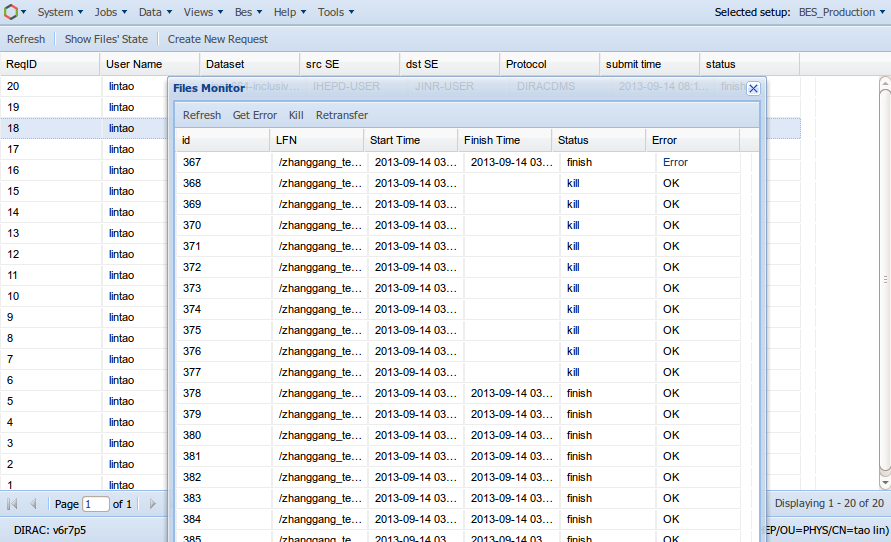
\includegraphics[width=.95\textwidth, keepaspectratio]{data/transreqlist-with-kill-retransfer.png}
\caption{\label{fig:ui}Transfer Request Management.
It shows the status of the dataset and the files in dataset.
It is in Bes$\to$Transfer$\to$Transfer Request in {\tt BESDIRAC}
web portal}
\end{minipage}
\hspace{.02\textwidth}
\begin{minipage}{.49\textwidth}
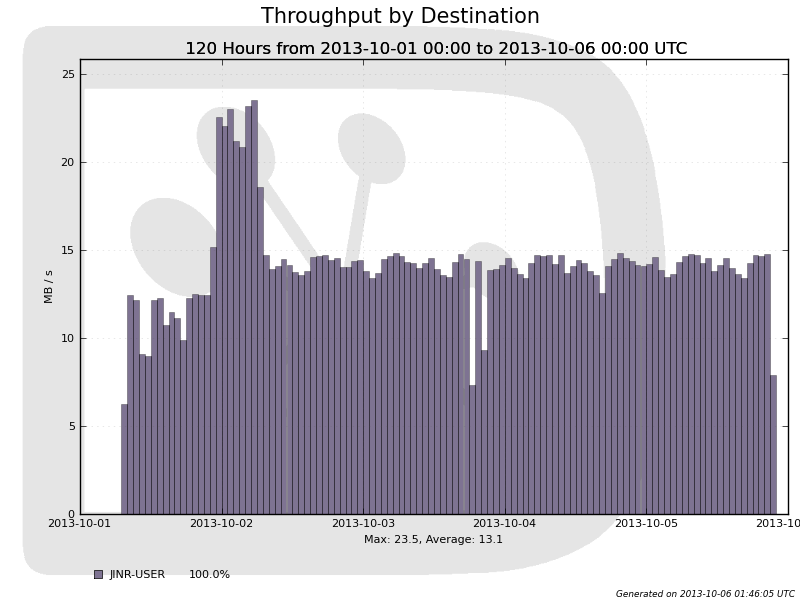
\includegraphics[width=.95\textwidth, keepaspectratio]{data/throughput-dest-1001-10-06.png}
\caption{\label{fig:throughput}Throughput from Oct.1 to Oct.6, 
average throughput is 15MB/s. This figure is generated in 
{\tt DIRAC} web portal automatically.}
\end{minipage}
\end{figure}

The main limitation of this system is the inefficiency because of 
the polling mechanism to check the status of the transfer processes.
It may waste CPU time. But this system is easy to extend.
Several transfer agents with multi-workers can be setup in different servers.
We will test this after several {\tt DIRAC} instances are installed.
Then, we will use one transfer database with several transfer agents
while the transfer agents will get the new requests from the database.
